\documentclass[8pt,aspectratio=169]{beamer}
\usetheme{Madrid}
\usepackage{graphicx}
\usepackage{booktabs}
\usepackage{adjustbox}
\usepackage{multicol}
\usepackage{amsmath}
\usepackage{amssymb}
\usepackage{tikz}
\usepackage{hyperref}
\usepackage{algorithm}
\usepackage{algorithmic}
\usepackage{colortbl}
\usepackage{pgfplots}
\pgfplotsset{compat=1.18}

% TikZ libraries for comics, diagrams, stakeholder maps
\usetikzlibrary{arrows.meta,positioning,shapes.callouts,shapes.geometric,decorations.pathreplacing}

% Color definitions
\definecolor{mlblue}{RGB}{0,102,204}
\definecolor{mlpurple}{RGB}{51,51,178}
\definecolor{mllavender}{RGB}{173,173,224}
\definecolor{mllavender2}{RGB}{193,193,232}
\definecolor{mllavender3}{RGB}{204,204,235}
\definecolor{mllavender4}{RGB}{214,214,239}
\definecolor{mlorange}{RGB}{255, 127, 14}
\definecolor{mlgreen}{RGB}{44, 160, 44}
\definecolor{mlred}{RGB}{214, 39, 40}
\definecolor{mlgray}{RGB}{127, 127, 127}
\definecolor{lightgray}{RGB}{240, 240, 240}
\definecolor{midgray}{RGB}{180, 180, 180}

% NEW COLORS for mini-lecture
\definecolor{dfteal}{RGB}{0,128,128}
\definecolor{dfred}{RGB}{180,30,30}

% Backward compatibility
\colorlet{MLPurple}{mlpurple}
\colorlet{MLBlue}{mlblue}
\colorlet{MLOrange}{mlorange}
\colorlet{MLGreen}{mlgreen}
\colorlet{MLRed}{mlred}
\colorlet{MLLavender}{mllavender}
\colorlet{MLGray}{mlgray}

% Theme colors (exact Madrid settings)
\setbeamercolor{palette primary}{bg=mllavender3,fg=mlpurple}
\setbeamercolor{palette secondary}{bg=mllavender2,fg=mlpurple}
\setbeamercolor{palette tertiary}{bg=mllavender,fg=white}
\setbeamercolor{palette quaternary}{bg=mlpurple,fg=white}
\setbeamercolor{structure}{fg=mlpurple}
\setbeamercolor{section in toc}{fg=mlpurple}
\setbeamercolor{subsection in toc}{fg=mlblue}
\setbeamercolor{title}{fg=mlpurple}
\setbeamercolor{frametitle}{fg=mlpurple,bg=mllavender3}
\setbeamercolor{block title}{bg=mllavender2,fg=mlpurple}
\setbeamercolor{block body}{bg=mllavender4,fg=black}
\setbeamertemplate{navigation symbols}{}
\setbeamertemplate{itemize items}[circle]
\setbeamertemplate{enumerate items}[default]
\setbeamersize{text margin left=5mm,text margin right=5mm}

% Footer
\setbeamertemplate{footline}{
  \leavevmode%
  \hbox{%
    \begin{beamercolorbox}[wd=.333333\paperwidth,ht=2.25ex,dp=1ex,center]{author in head/foot}%
      \usebeamerfont{author in head/foot}Methods and Algorithms
    \end{beamercolorbox}%
    \begin{beamercolorbox}[wd=.333333\paperwidth,ht=2.25ex,dp=1ex,center]{title in head/foot}%
      \usebeamerfont{title in head/foot}MSc Data Science
    \end{beamercolorbox}%
    \begin{beamercolorbox}[wd=.333333\paperwidth,ht=2.25ex,dp=1ex,right]{date in head/foot}%
      \usebeamerfont{date in head/foot}\insertframenumber{} / \inserttotalframenumber\hspace*{2ex}
    \end{beamercolorbox}}%
  \vskip0pt%
}

\newcommand{\bottomnote}[1]{%
\vfill
\vspace{-2mm}
\textcolor{mllavender2}{\rule{\textwidth}{0.4pt}}
\vspace{1mm}
\footnotesize
\textbf{#1}
}

\newenvironment{compactlist}{%
  \begin{itemize}%
    \setlength{\itemsep}{2pt}%
    \setlength{\parskip}{0pt}%
    \setlength{\parsep}{0pt}%
}{%
  \end{itemize}%
}

\newcommand{\highlight}[1]{\textcolor{mlorange}{\textbf{#1}}}
\newcommand{\mathbold}[1]{\boldsymbol{#1}}

% ============================================================
\title[Classification \& Decomposition Mini-Lecture]{Classification \& Data Decomposition}
\subtitle{Mini-Lecture: Sorting, Grouping, and Compressing Data}
\author{Methods and Algorithms}
\institute{MSc Data Science}
\date{}

\begin{document}

% ----------------------------------------------------------
% Slide 1: Title
% ----------------------------------------------------------
\begin{frame}[plain]
\vfill
\titlepage
\vfill
\end{frame}

% ----------------------------------------------------------
% Slide 2: XKCD Opening
% ----------------------------------------------------------
\begin{frame}{The Neural Net Knows Best}
\centering
\includegraphics[height=0.65\textheight]{images/2173_trained_a_neural_net.png}

\bottomnote{XKCD \#2173 by Randall Munroe (CC BY-NC 2.5)}
\end{frame}

% ----------------------------------------------------------
% Slide 3: Classification
% ----------------------------------------------------------
\begin{frame}{Classification: Assigning Labels}
\begin{columns}[T]
\begin{column}{0.55\textwidth}
\begin{compactlist}
\item Predict a \highlight{discrete class}: $y \in \{0,1,\ldots,K\}$
\item Binary: default / no-default; Multiclass: sector label
\item A \highlight{decision boundary} separates classes in feature space
\item Full treatment in L02 (logistic regression) and L04 (random forests)
\end{compactlist}
\end{column}
\begin{column}{0.42\textwidth}
\centering
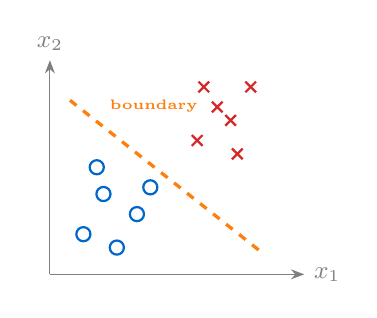
\begin{tikzpicture}[scale=0.85, >=Stealth]
  \draw[->,mlgray] (0,0) -- (3.8,0) node[right]{\small $x_1$};
  \draw[->,mlgray] (0,0) -- (0,3.2) node[above]{\small $x_2$};
  % Class 0: circles
  \foreach \x/\y in {0.5/0.6, 0.8/1.2, 1.0/0.4, 1.3/0.9, 0.7/1.6, 1.5/1.3}
    \draw[mlblue,thick] (\x,\y) circle(3pt);
  % Class 1: crosses
  \foreach \x/\y in {2.2/2.0, 2.5/2.5, 2.8/1.8, 3.0/2.8, 2.3/2.8, 2.7/2.3}
  {
    \draw[mlred,thick] (\x-0.08,\y-0.08) -- (\x+0.08,\y+0.08);
    \draw[mlred,thick] (\x-0.08,\y+0.08) -- (\x+0.08,\y-0.08);
  }
  % Decision boundary
  \draw[mlorange,very thick,dashed] (0.3,2.6) -- (3.2,0.3)
        node[pos=0.15,above right,font=\tiny\bfseries,mlorange]{boundary};
\end{tikzpicture}
\end{column}
\end{columns}

\bottomnote{Classification is the most common ML task in banking --- credit scoring, fraud, compliance.}
\end{frame}

% ----------------------------------------------------------
% Slide 4: How Classifiers Decide
% ----------------------------------------------------------
\begin{frame}{How Classifiers Decide}
\begin{compactlist}
\item \highlight{Logistic regression}: estimates $P(y{=}1 \mid \mathbf{X})$, threshold at 0.5 (L02)
\item \highlight{KNN}: majority vote among $K$ nearest neighbours (L03)
\item \highlight{Decision tree}: recursive if-then splits on features (L04)
\item Each algorithm creates a \emph{different} decision boundary shape
\end{compactlist}

\vspace{3mm}
\begin{block}{Choosing a Classifier}
No single method dominates all problems --- the ``best'' classifier depends on
data size, feature types, and interpretability requirements.
\end{block}

\bottomnote{This is definition-level orientation --- full formulas and derivations come in L02--L04.}
\end{frame}

% ----------------------------------------------------------
% Slide 5: Evaluating Classifiers
% ----------------------------------------------------------
\begin{frame}{Evaluating Classifiers}
\begin{columns}[T]
\begin{column}{0.55\textwidth}
\begin{compactlist}
\item \highlight{Accuracy} can be misleading: 99\% on 1\% fraud = useless model
\item \highlight{Confusion matrix}: TP, FP, TN, FN
\item Precision $= \frac{TP}{TP+FP}$ \quad (of predicted positives, how many correct?)
\item Recall $= \frac{TP}{TP+FN}$ \quad (of actual positives, how many found?)
\end{compactlist}
\end{column}
\begin{column}{0.42\textwidth}
\centering
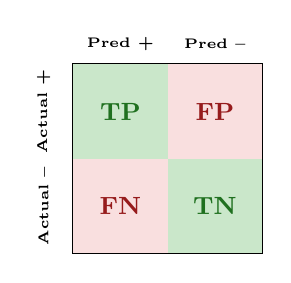
\begin{tikzpicture}[scale=0.75]
  % grid
  \draw[thick] (0,0) rectangle (3.2,3.2);
  \draw[thick] (1.6,0) -- (1.6,3.2);
  \draw[thick] (0,1.6) -- (3.2,1.6);
  % cells
  \fill[mlgreen!25] (0,1.6) rectangle (1.6,3.2);   % TP
  \fill[mlred!15]   (1.6,1.6) rectangle (3.2,3.2);  % FP
  \fill[mlred!15]   (0,0) rectangle (1.6,1.6);       % FN
  \fill[mlgreen!25] (1.6,0) rectangle (3.2,1.6);    % TN
  % labels inside
  \node[font=\small\bfseries,mlgreen!70!black] at (0.8,2.4) {TP};
  \node[font=\small\bfseries,mlred!70!black]   at (2.4,2.4) {FP};
  \node[font=\small\bfseries,mlred!70!black]   at (0.8,0.8) {FN};
  \node[font=\small\bfseries,mlgreen!70!black] at (2.4,0.8) {TN};
  % axis labels
  \node[font=\tiny\bfseries,rotate=90] at (-0.5,2.4) {Actual +};
  \node[font=\tiny\bfseries,rotate=90] at (-0.5,0.8) {Actual --};
  \node[font=\tiny\bfseries] at (0.8,3.55) {Pred +};
  \node[font=\tiny\bfseries] at (2.4,3.55) {Pred --};
\end{tikzpicture}
\end{column}
\end{columns}

\bottomnote{In fraud detection, recall matters most --- missing a fraud case is far costlier than a false alarm.}
\end{frame}

% ----------------------------------------------------------
% Slide 6: Clustering
% ----------------------------------------------------------
\begin{frame}{Clustering: Grouping Without Labels}
\begin{columns}[T]
\begin{column}{0.55\textwidth}
\begin{compactlist}
\item Partition $n$ observations into $K$ groups based on \highlight{similarity}
\item \highlight{K-Means}: assign to nearest centroid, update centroids, repeat (definition only --- full algorithm in L03)
\item Evaluate with \highlight{inertia} (within-cluster sum of squares) and \highlight{silhouette score}
\item Finance: segment retail banking customers by spending behaviour
\end{compactlist}
\end{column}
\begin{column}{0.42\textwidth}
\centering
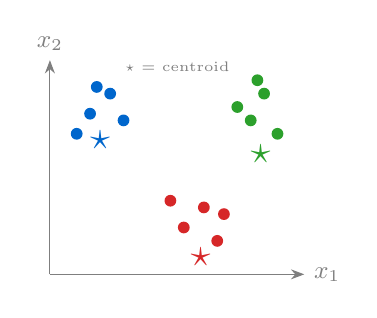
\begin{tikzpicture}[scale=0.85, >=Stealth]
  \draw[->,mlgray] (0,0) -- (3.8,0) node[right]{\small $x_1$};
  \draw[->,mlgray] (0,0) -- (0,3.2) node[above]{\small $x_2$};
  % Cluster 1
  \foreach \x/\y in {0.6/2.4, 0.9/2.7, 0.4/2.1, 1.1/2.3, 0.7/2.8}
    \fill[mlblue] (\x,\y) circle(2.5pt);
  \node[mlblue,font=\Large] at (0.75,2.0) {$\star$};
  % Cluster 2
  \foreach \x/\y in {2.0/0.7, 2.3/1.0, 2.5/0.5, 1.8/1.1, 2.6/0.9}
    \fill[mlred] (\x,\y) circle(2.5pt);
  \node[mlred,font=\Large] at (2.25,0.25) {$\star$};
  % Cluster 3
  \foreach \x/\y in {3.0/2.3, 3.2/2.7, 2.8/2.5, 3.4/2.1, 3.1/2.9}
    \fill[mlgreen] (\x,\y) circle(2.5pt);
  \node[mlgreen,font=\Large] at (3.15,1.8) {$\star$};
  % legend
  \node[font=\tiny,mlgray] at (1.9,3.1) {$\star$ = centroid};
\end{tikzpicture}
\end{column}
\end{columns}

\bottomnote{K-Means is the most widely used clustering algorithm --- simple, fast, and surprisingly effective.}
\end{frame}

% ----------------------------------------------------------
% Slide 7: Dimensionality Reduction
% ----------------------------------------------------------
\begin{frame}{Dimensionality Reduction}
\begin{columns}[T]
\begin{column}{0.55\textwidth}
\begin{compactlist}
\item High-dimensional data ($p \gg 3$) is hard to visualize and model
\item \highlight{PCA}: project onto directions of maximum variance (definition only --- full derivation in L05)
\item \highlight{t-SNE}: preserve local neighbourhoods in 2D (L05)
\item Goal: reduce $p$ features to $k \ll p$ while retaining information
\end{compactlist}
\end{column}
\begin{column}{0.42\textwidth}
\centering
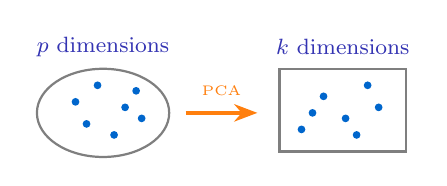
\begin{tikzpicture}[scale=0.7, >=Stealth]
  % 3D cloud (simplified)
  \draw[mlgray,thick] (0,1) ellipse (1.2 and 0.8);
  \foreach \x/\y in {-0.5/1.2, 0.2/0.6, 0.6/1.4, -0.3/0.8, 0.4/1.1, -0.1/1.5, 0.7/0.9}
    \fill[mlblue] (\x,\y) circle(2pt);
  \node[font=\footnotesize,mlpurple] at (0,2.2) {$p$ dimensions};
  % arrow
  \draw[->,very thick,mlorange] (1.5,1) -- (2.8,1);
  \node[font=\tiny,mlorange] at (2.15,1.4) {PCA};
  % 2D plane
  \draw[mlgray,thick] (3.2,0.3) -- (5.5,0.3) -- (5.5,1.8) -- (3.2,1.8) -- cycle;
  \foreach \x/\y in {3.6/0.7, 4.0/1.3, 4.4/0.9, 4.8/1.5, 3.8/1.0, 4.6/0.6, 5.0/1.1}
    \fill[mlblue] (\x,\y) circle(2pt);
  \node[font=\footnotesize,mlpurple] at (4.35,2.2) {$k$ dimensions};
\end{tikzpicture}
\end{column}
\end{columns}

\bottomnote{PCA is the workhorse of dimensionality reduction --- it connects directly to eigenvalues from P01.}
\end{frame}

% ----------------------------------------------------------
% Slide 8: The Decomposition Perspective
% ----------------------------------------------------------
\begin{frame}{The Decomposition Perspective}
\begin{compactlist}
\item \highlight{Decomposition} = breaking a complex signal into simpler components
\item \highlight{SVD}: $\mathbf{X} \approx \mathbf{U}\boldsymbol{\Sigma}\mathbf{V}^\top$ (truncated to rank $k$)
\item Factor analysis: discover \highlight{latent factors} driving observed correlations
\item Finance: stock return $=$ market factor $+$ sector factor $+$ idiosyncratic noise
\end{compactlist}

\vspace{3mm}
\[
\underbrace{\mathbf{X}}_{n \times p}
\;\approx\;
\underbrace{\mathbf{U}}_{n \times k}
\;\underbrace{\boldsymbol{\Sigma}}_{k \times k}
\;\underbrace{\mathbf{V}^\top}_{k \times p}
\qquad (k \ll p)
\]

\vspace{1mm}
\begin{block}{Why It Matters}
PCA is a special case of SVD applied to centred data --- L05 builds on this foundation.
\end{block}

\bottomnote{Decomposition unifies PCA, factor models, and matrix approximation under one framework.}
\end{frame}

% ----------------------------------------------------------
% Slide 9: Finance Pipeline
% ----------------------------------------------------------
\begin{frame}{Finance: Putting It All Together}
\begin{columns}[T]
\begin{column}{0.55\textwidth}
\begin{compactlist}
\item \highlight{Classification}: credit scoring (L02), fraud detection (L04)
\item \highlight{Clustering}: customer segmentation, market regime detection (L03)
\item \highlight{Decomposition}: PCA on 50 stock returns $\to$ 3 risk factors (L05)
\end{compactlist}

\vspace{2mm}
\begin{block}{Combined Workflow}
Decompose $\to$ Cluster $\to$ Classify $\to$ Decide
\end{block}
\end{column}
\begin{column}{0.42\textwidth}
\centering
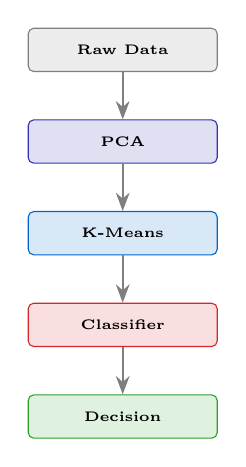
\begin{tikzpicture}[node distance=0.6cm, >=Stealth,
  pbox/.style={draw,rounded corners=2pt,minimum width=2.4cm,
               minimum height=0.55cm,font=\tiny\bfseries,align=center}]
  \node[pbox,fill=mlgray!15,draw=mlgray]     (raw) {Raw Data};
  \node[pbox,fill=mlpurple!15,draw=mlpurple,below=of raw] (pca) {PCA};
  \node[pbox,fill=mlblue!15,draw=mlblue,below=of pca]     (km)  {K-Means};
  \node[pbox,fill=mlred!15,draw=mlred,below=of km]        (cls) {Classifier};
  \node[pbox,fill=mlgreen!15,draw=mlgreen,below=of cls]   (dec) {Decision};
  \draw[->,thick,mlgray] (raw) -- (pca);
  \draw[->,thick,mlgray] (pca) -- (km);
  \draw[->,thick,mlgray] (km)  -- (cls);
  \draw[->,thick,mlgray] (cls) -- (dec);
\end{tikzpicture}
\end{column}
\end{columns}

\bottomnote{This pipeline appears throughout L01--L06 --- each lecture fills in one piece of the puzzle.}
\end{frame}

% ----------------------------------------------------------
% Slide 10: Summary
% ----------------------------------------------------------
\begin{frame}{Summary: Classification, Clustering, Decomposition}
\begin{enumerate}
\setlength{\itemsep}{6pt}
\item \highlight{Classification} assigns discrete labels --- evaluate with precision and recall, not just accuracy
\item \highlight{Clustering} (K-Means) groups data without labels --- full algorithm in L03
\item \highlight{Dimensionality reduction} (PCA, t-SNE) compresses features --- derivation in L05
\item Finance \highlight{combines all three}: decompose $\to$ cluster $\to$ classify $\to$ decide
\end{enumerate}

\vspace{4mm}
\begin{block}{You Are Ready}
With P01--P03 complete, you have the vocabulary and intuition for L01--L06.
\end{block}

\bottomnote{These three concepts --- classify, cluster, decompose --- are the verbs of applied machine learning.}
\end{frame}

\end{document}
